% Options for packages loaded elsewhere
\PassOptionsToPackage{unicode}{hyperref}
\PassOptionsToPackage{hyphens}{url}
%
\documentclass[
]{article}
\usepackage{lmodern}
\usepackage{amssymb,amsmath}
\usepackage{ifxetex,ifluatex}
\ifnum 0\ifxetex 1\fi\ifluatex 1\fi=0 % if pdftex
  \usepackage[T1]{fontenc}
  \usepackage[utf8]{inputenc}
  \usepackage{textcomp} % provide euro and other symbols
\else % if luatex or xetex
  \usepackage{unicode-math}
  \defaultfontfeatures{Scale=MatchLowercase}
  \defaultfontfeatures[\rmfamily]{Ligatures=TeX,Scale=1}
\fi
% Use upquote if available, for straight quotes in verbatim environments
\IfFileExists{upquote.sty}{\usepackage{upquote}}{}
\IfFileExists{microtype.sty}{% use microtype if available
  \usepackage[]{microtype}
  \UseMicrotypeSet[protrusion]{basicmath} % disable protrusion for tt fonts
}{}
\makeatletter
\@ifundefined{KOMAClassName}{% if non-KOMA class
  \IfFileExists{parskip.sty}{%
    \usepackage{parskip}
  }{% else
    \setlength{\parindent}{0pt}
    \setlength{\parskip}{6pt plus 2pt minus 1pt}}
}{% if KOMA class
  \KOMAoptions{parskip=half}}
\makeatother
\usepackage{xcolor}
\IfFileExists{xurl.sty}{\usepackage{xurl}}{} % add URL line breaks if available
\IfFileExists{bookmark.sty}{\usepackage{bookmark}}{\usepackage{hyperref}}
\hypersetup{
  pdftitle={Savev David 14057},
  hidelinks,
  pdfcreator={LaTeX via pandoc}}
\urlstyle{same} % disable monospaced font for URLs
\usepackage[margin=1in]{geometry}
\usepackage{graphicx,grffile}
\makeatletter
\def\maxwidth{\ifdim\Gin@nat@width>\linewidth\linewidth\else\Gin@nat@width\fi}
\def\maxheight{\ifdim\Gin@nat@height>\textheight\textheight\else\Gin@nat@height\fi}
\makeatother
% Scale images if necessary, so that they will not overflow the page
% margins by default, and it is still possible to overwrite the defaults
% using explicit options in \includegraphics[width, height, ...]{}
\setkeys{Gin}{width=\maxwidth,height=\maxheight,keepaspectratio}
% Set default figure placement to htbp
\makeatletter
\def\fps@figure{htbp}
\makeatother
\setlength{\emergencystretch}{3em} % prevent overfull lines
\providecommand{\tightlist}{%
  \setlength{\itemsep}{0pt}\setlength{\parskip}{0pt}}
\setcounter{secnumdepth}{-\maxdimen} % remove section numbering

\title{Savev David 14057}
\author{}
\date{\vspace{-2.5em}}

\begin{document}
\maketitle

Gender GAP ``STEM'' degrees

The purpose of this document, is to show the existing gender gap in the
italian degrees being parts of the so called ``Science, Technology,
Engineering and Mathematics'' group; the dataset was downloaded from the
official Dati Ustat website: \url{http://dati.ustat.miur.it/dataset/}
The selected dataset contains the number of gruadates in the time period
2012-2018 divided by degree type, level of instruction (Bachelor,
Master), university and gender.

Data pre-processing

Since the dataset uses ``;'' character as delimiter (the ``,'' is used
as punctuation character), read\_csv2 is the most suitable command in
order to read in an appropriate way the file.

\begin{verbatim}
## # A tibble: 19,022 x 10
##     ANNO AteneoCOD AteneoNOME AteneoREGIONE AteneoAREAGEO CorsoTIPO COD_FoET2013
##    <dbl> <chr>     <chr>      <chr>         <chr>         <chr>     <chr>       
##  1  2018 00101     "Torino -~ Piemonte      NORD-OVEST    Laurea    01          
##  2  2018 00101     "Torino -~ Piemonte      NORD-OVEST    Laurea    01          
##  3  2018 00101     "Torino -~ Piemonte      NORD-OVEST    Laurea    02          
##  4  2018 00101     "Torino -~ Piemonte      NORD-OVEST    Laurea    02          
##  5  2018 00101     "Torino -~ Piemonte      NORD-OVEST    Laurea    03          
##  6  2018 00101     "Torino -~ Piemonte      NORD-OVEST    Laurea    03          
##  7  2018 00101     "Torino -~ Piemonte      NORD-OVEST    Laurea    04          
##  8  2018 00101     "Torino -~ Piemonte      NORD-OVEST    Laurea    04          
##  9  2018 00101     "Torino -~ Piemonte      NORD-OVEST    Laurea    05          
## 10  2018 00101     "Torino -~ Piemonte      NORD-OVEST    Laurea    05          
## # ... with 19,012 more rows, and 3 more variables: DESC_FoET2013 <chr>,
## #   Genere <chr>, LAU <dbl>
\end{verbatim}

After a first pre-processing of the .csv file (renaming of entries and
columns names with suitable names) and dropping off unesuful columns,
the dataframe results in a tidy version, in the following way:

\begin{verbatim}
## # A tibble: 19,022 x 8
##     Year University     Region  GeoArea EducationLevel Degree      Gender Number
##    <dbl> <chr>          <chr>   <chr>   <chr>          <chr>       <chr>   <dbl>
##  1  2018 "Torino - Uni~ Piemon~ North-~ Bachelor       Education   F         293
##  2  2018 "Torino - Uni~ Piemon~ North-~ Bachelor       Education   M          24
##  3  2018 "Torino - Uni~ Piemon~ North-~ Bachelor       Arts and h~ F         833
##  4  2018 "Torino - Uni~ Piemon~ North-~ Bachelor       Arts and h~ M         306
##  5  2018 "Torino - Uni~ Piemon~ North-~ Bachelor       Social sci~ F        1034
##  6  2018 "Torino - Uni~ Piemon~ North-~ Bachelor       Social sci~ M         711
##  7  2018 "Torino - Uni~ Piemon~ North-~ Bachelor       Business, ~ F         654
##  8  2018 "Torino - Uni~ Piemon~ North-~ Bachelor       Business, ~ M         684
##  9  2018 "Torino - Uni~ Piemon~ North-~ Bachelor       Natural sc~ F         422
## 10  2018 "Torino - Uni~ Piemon~ North-~ Bachelor       Natural sc~ M         304
## # ... with 19,012 more rows
\end{verbatim}

Data Visualization

In year 2018, the total number of italian graduates was: 326244, where
140072 male and 186172 female; that means that the ratio male-female
could be reppresented by the following piechart:

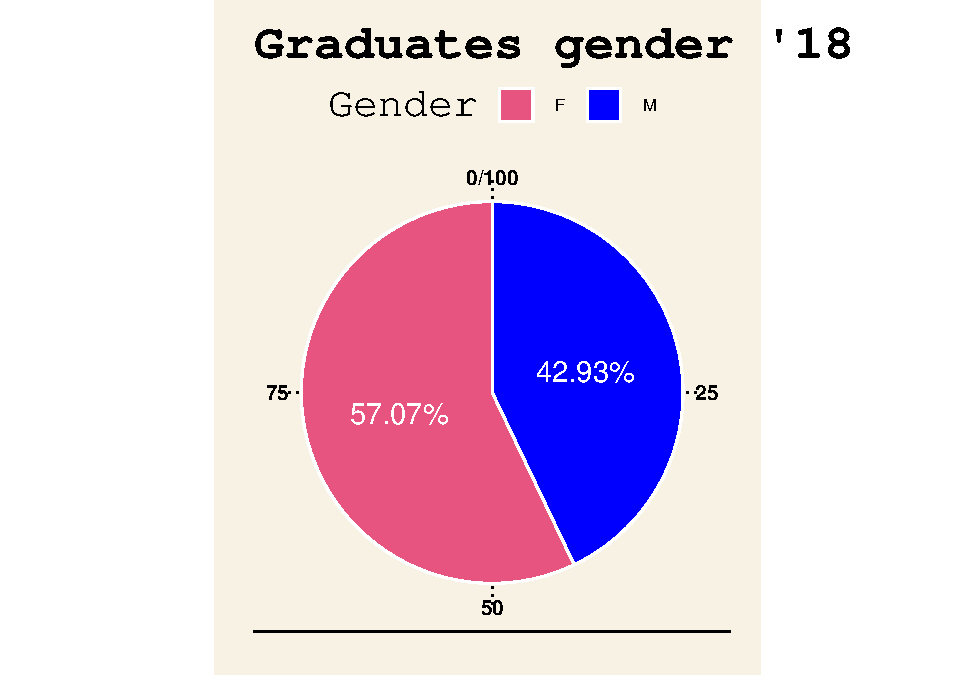
\includegraphics{g_gap_stem_files/figure-latex/unnamed-chunk-3-1.pdf}

The degree type of the graduates in year 2018 is shown through the
following bar-chart and is also ordered in descending order:

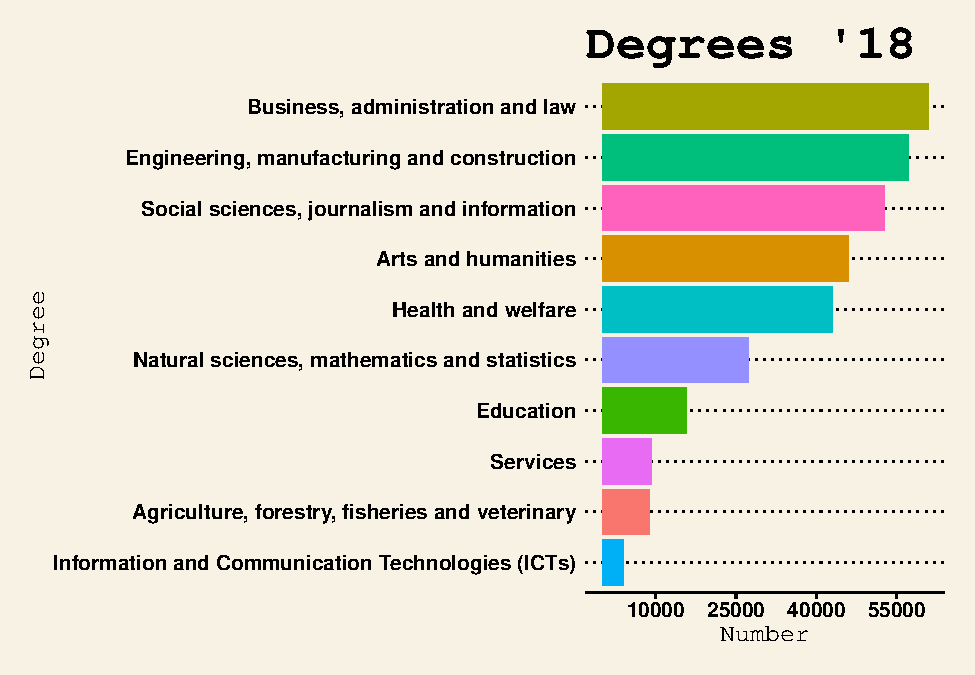
\includegraphics{g_gap_stem_files/figure-latex/unnamed-chunk-4-1.pdf}

For what concerns the STEM disciplines, We can recognize that they were
grouped inside the dataset in three main sectors:

Engineering, Manufactoring and Construction;

Natural Sciences, Math and Statistics;

ICTs;

Although the total number of female graduates is bigger, the amount of
female gruaduates in the ``S.T.E.M.'' disciplines in year 2018 is pretty
small, since from a total of 88391, only 34386 are female:

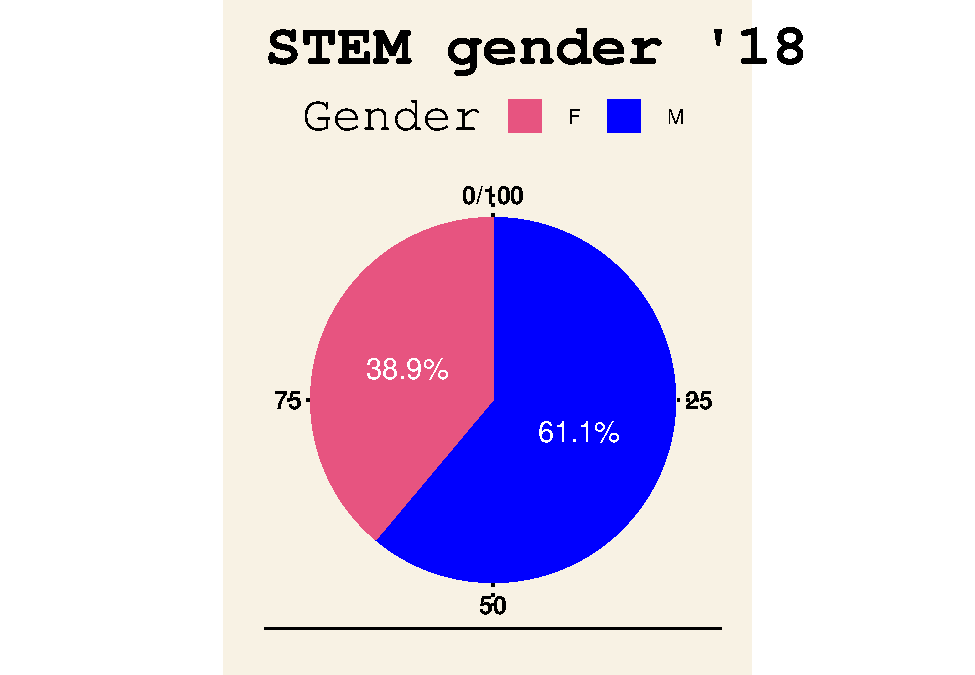
\includegraphics{g_gap_stem_files/figure-latex/unnamed-chunk-5-1.pdf}

By plotting the number of STEM graduates by gender, We can clearly
recognize were the quantitive gap male-female actually resides:

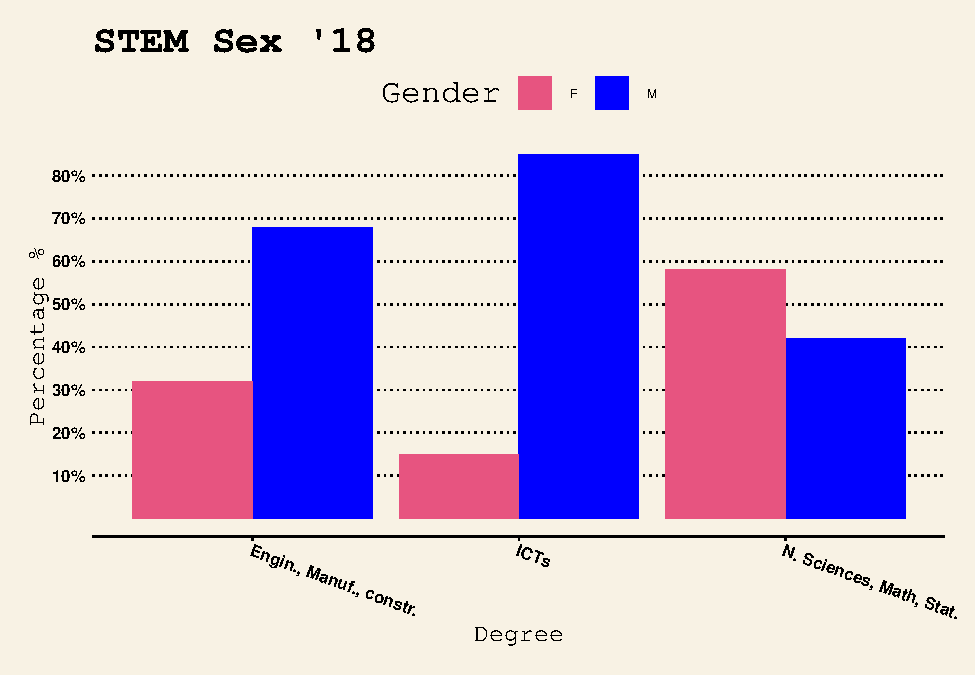
\includegraphics{g_gap_stem_files/figure-latex/unnamed-chunk-6-1.pdf}

By following the trend of the number of female gruaduates in STEM
disciplines from 2012 till 2018, We can see that the percentage has
slightly dropped from 40.098\% to 38.902\% as it can be denoticed from
the following linechart:

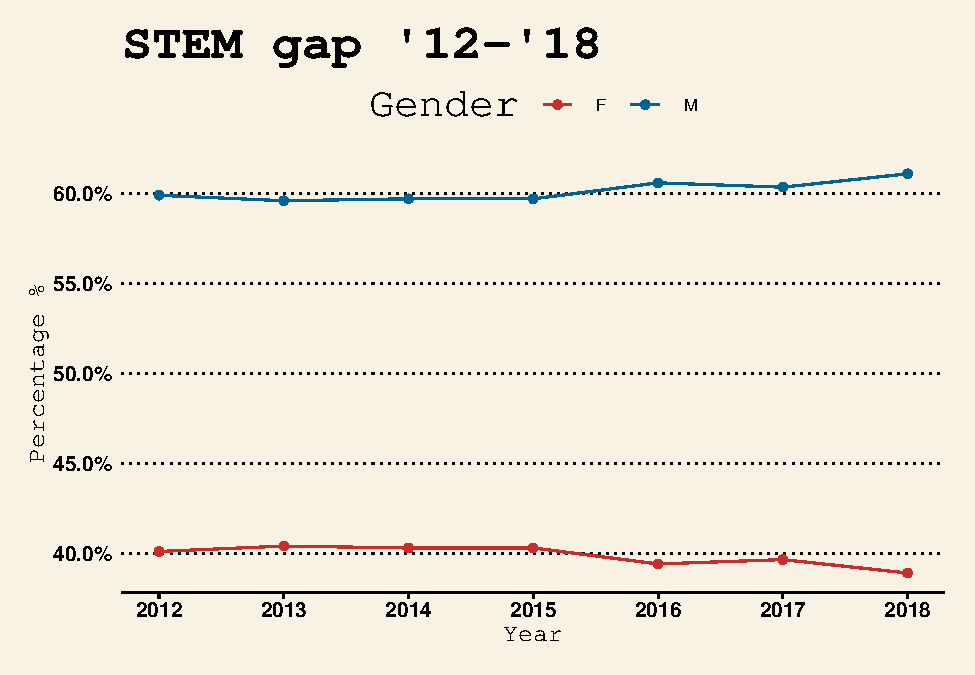
\includegraphics{g_gap_stem_files/figure-latex/unnamed-chunk-7-1.pdf}

By analyzing the STEM gender gap in the last years, We can recognize a
specific pattern that manifests itself every year: Northern Italy has
the smallest percentage of female graduates in whole Italy..

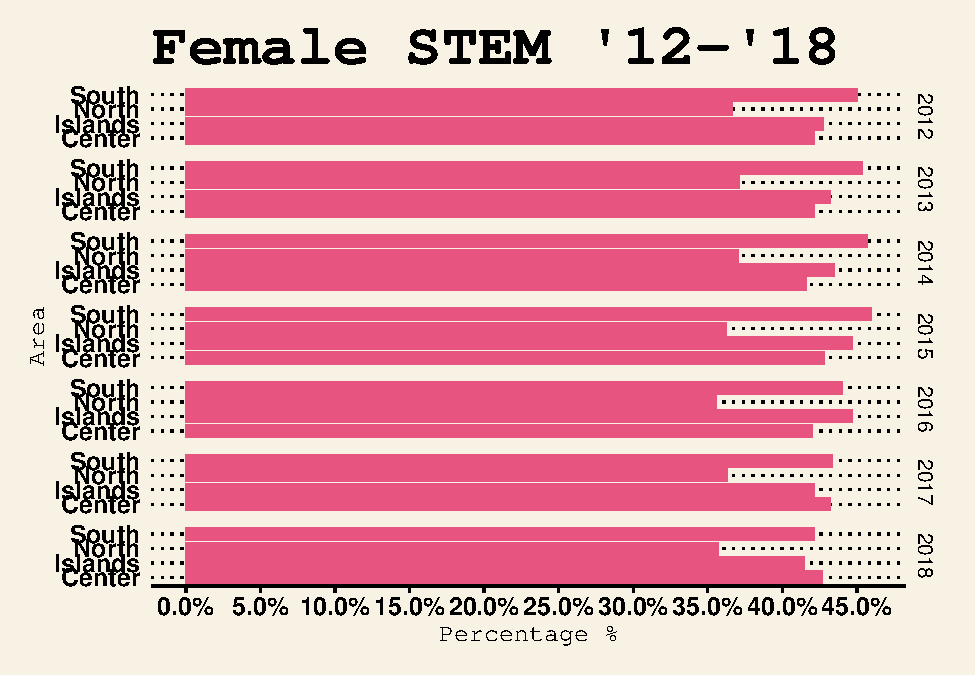
\includegraphics{g_gap_stem_files/figure-latex/unnamed-chunk-8-1.pdf}

Since among the period 2012-2018 We have a similar pattern (Northern
Italy with the smallest percentages, Southern or Center Italy usually
with the highest), We could plot the mean of female STEM graduates
ordered by region in the last 6 years (2012-2018):

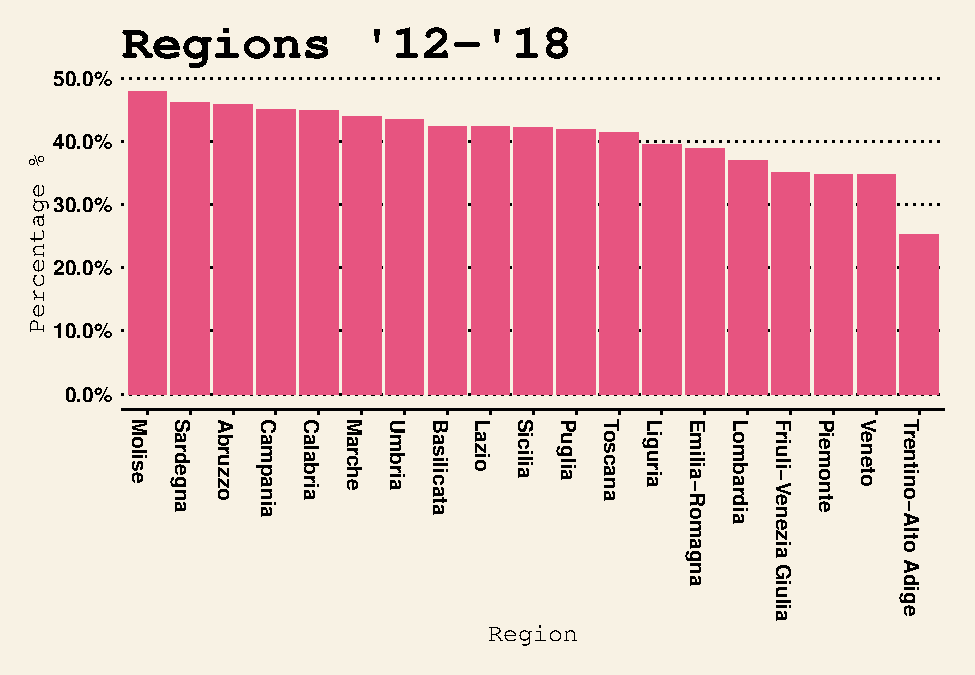
\includegraphics{g_gap_stem_files/figure-latex/unnamed-chunk-9-1.pdf}

By the way, mapping the previous barchart to an italian map, could be
hovewer more expressive (Valle d'Aosta has no relevant data since there
are no ``STEM'' faculties):

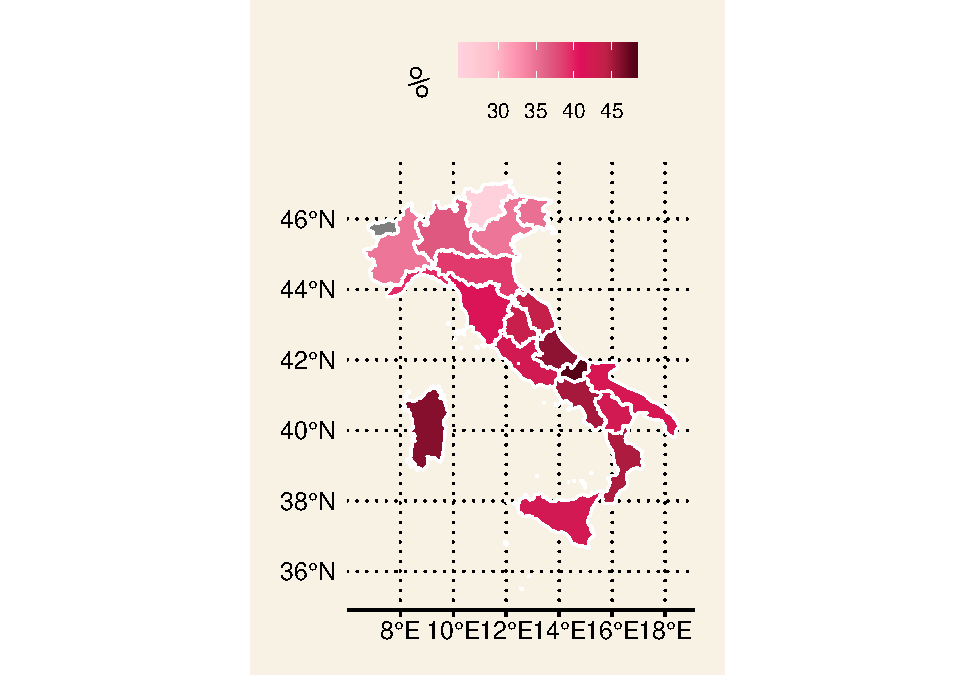
\includegraphics{g_gap_stem_files/figure-latex/unnamed-chunk-10-1.pdf}

\end{document}
